\chapter{蚂蚁的数学}

作为当今世界上最为成功的物种之一,蚂蚁虽然只有大约 25 万个神经元细胞,但其复杂的生物学行为却令人瞩目。
特别是其归巢行为,已经成为了数学和生物学研究的重要课题。\cite{Wehner2003DesertAN}
这不仅证明了即使是“简单”的生物也具有出奇不意的数学能力,而且还为我们理解数学如何根植于自然界提供了宝贵的线索。

\begin{figure}[ht]\centering
\resizebox{0.5\textwidth}{!}{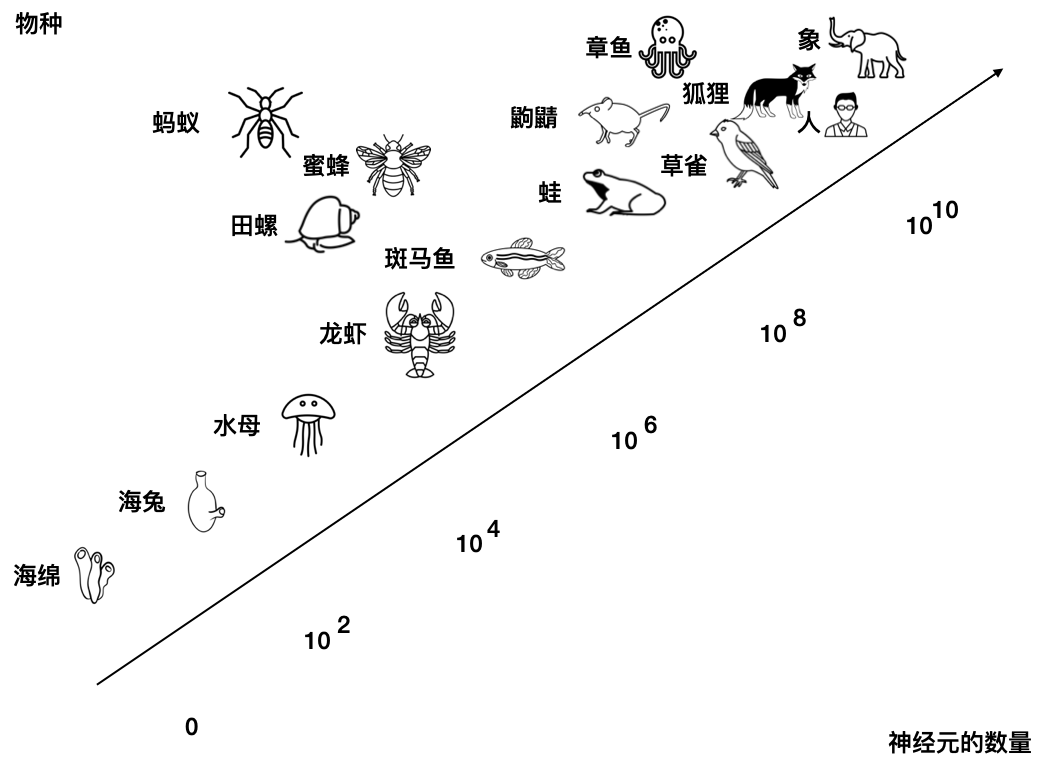
\includegraphics{images/01_01-species-neuron}}
\caption{物种与神经元数量}
\end{figure}

Wehner 等人在 2003 年的一项引人注目的实验中发现了令人惊讶的事实。沙漠蚁在归巢时,并不依赖于地理空间的绝对位置,
而是采用了一种被称为“路径积分”的策略。\cite{Wehner2003DesertAN}简而言之,这些蚂蚁会在移动过程中不断记录自己的方向和距离,
然后利用这些信息来确定回到巢穴的最直接路径。这一发现不仅展示了蚂蚁在数学方面的先天能力,也进一步证实了数学能力是生物界中普遍存在的现象。

在 Wehner 的实验 A 中,沙漠蚁在自由行走中会径直返巢。对照实验 B 则设置了挡板(图 \ref{fig:ant-navi} 中灰色线),沙漠蚁被挡板阻挡不得不绕行;但是一旦挡板消失,它们就会径直返巢。
我们能从实验 B 结果的图示上,清晰而直接地看到沙漠蚁有三角学角度的解算能力。
Wittlinger 在 2006 年的实验,也进一步说明沙漠蚁有计步能力。\cite{Wittlinger2006TheAO}
这些数学能力蕴含在生物的本能中,不是以符号的形式存在的。

\begin{figure}[ht]\centering
\resizebox{0.5\textwidth}{!}{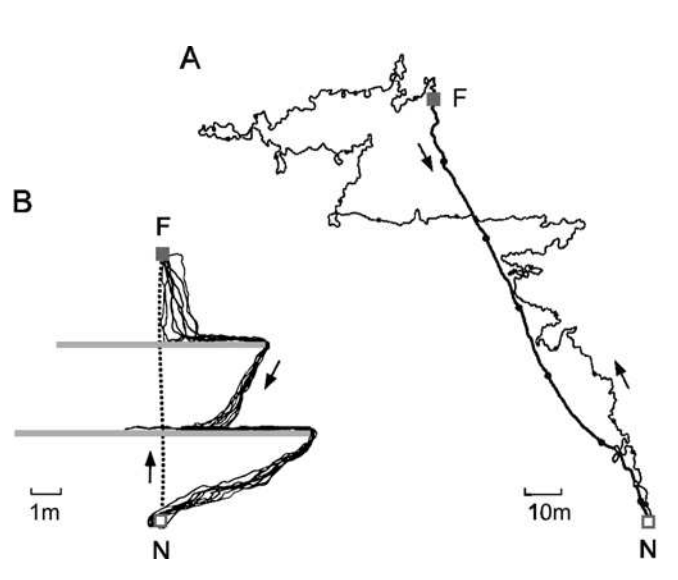
\includegraphics{images/01_02-ant-navi}}
\caption{关于蚂蚁归巢行为的实验}\label{fig:ant-navi}
\end{figure}

在导航能力的研究中,动物大脑的神经科学机制也是一个热门话题。科学家们已经区分了两种主要的动物导航原理:
一种是以自我为中心的导航(也就是“自我中心式的”或egocentric),另一种是依赖于外部地标的导航(也就是“地标式的”或geocentric)。
这两种导航方式背后都有复杂的神经科学机制。对于高等的动物,位置细胞和网格细胞在动物大脑中起到了关键作用,它们为动物提供了空间定位的神经科学基础
\cite{Moser2008PlaceCG}。这一发现不仅增加了我们对动物数学能力的理解,也为探究人类数学思维提供了新的视角。

从这些研究中,我们可以推测,人类数学的根源很可能是生物在数亿年的演化过程中逐渐形成的数学能力。
这种能力不仅仅是生物为了适应环境而演化出来的,它背后的神经机制还是我们数学直觉的基础。但这引出了一些更为引人入胜的问题:
人类的数学思维能否,以及如何,超越这种深植于我们基因的原始数学能力?人类原始的数学直觉是如何转化为更高级的数学概念,例如无穷、概率或者高维几何?
再如,我们是否可以,设计一个实验观察动物大脑在高维数字虚拟空间中的活动过程?这一类的探索不仅可以成为一个严肃的科学问题,
也触及了哲学和文化的多个层面,会帮助我们进一步理解人类数学思维和数学实在的本质。

\bibliographystyle{apalike2}
\bibliography{biblio/chp01}
